\documentclass[11pt]{article}
\usepackage{geometry}
\usepackage[utf8]{inputenc}
\usepackage[english]{babel}
\usepackage{amsmath}
\usepackage{amssymb}
\usepackage{amsfonts}
\usepackage[pdftex, dvipsnames]{xcolor}
\usepackage[
    colorlinks=false,
    linkbordercolor=pink
]{hyperref}
\usepackage{fancyhdr}
\usepackage{datetime}
\usepackage{xargs}
\usepackage{ccicons}
\usepackage{mdframed}
\usepackage{caption}
\usepackage{cancel}
\usepackage[nottoc]{tocbibind}
\usepackage[outputdir=.texpadtmp]{minted}

% ==== License =====
\usepackage[
    type={CC}, 
    modifier={by-nc-sa}, 
    version={4.0},
]{doclicense}

% ==== todo notes ====
\usepackage[
    colorinlistoftodos,
    prependcaption,
    textsize=tiny
]{todonotes}
\newcommandx{\note}[2][1=]{\todo[linecolor=Thistle,backgroundcolor=Thistle!25,bordercolor=Thistle,#1]{#2}}
\newcommandx{\unsure}[2][1=]{\todo[linecolor=red,backgroundcolor=red!25,bordercolor=red,#1]{#2}}
\newcommandx{\change}[2][1=]{\todo[linecolor=blue,backgroundcolor=blue!25,bordercolor=blue,#1]{#2}}
\newcommandx{\info}[2][1=]{\todo[linecolor=OliveGreen,backgroundcolor=OliveGreen!25,bordercolor=OliveGreen,#1]{#2}}

% General
\newcommand{\mc}[1]{\mathcal{#1}}

% Math Bold Font, Vector Notations
\newcommand{\ba}{\mathbf{a}}
\newcommand{\bb}{\mathbf{b}}
\newcommand{\bc}{\mathbf{c}}
\newcommand{\bd}{\mathbf{d}}
\newcommand{\be}{\mathbf{e}}
\renewcommand{\bf}{\mathbf{f}}
\newcommand{\bg}{\mathbf{g}}
\newcommand{\bh}{\mathbf{h}}
\newcommand{\bi}{\mathbf{i}}
\newcommand{\bj}{\mathbf{j}}
\newcommand{\bk}{\mathbf{k}}
\newcommand{\bl}{\mathbf{l}}
\newcommand{\bm}{\mathbf{m}}
\newcommand{\bn}{\mathbf{n}}
\newcommand{\bo}{\mathbf{o}}
\newcommand{\bp}{\mathbf{p}}
\newcommand{\bq}{\mathbf{q}}
\newcommand{\br}{\mathbf{r}}
\newcommand{\bs}{\mathbf{s}}
\newcommand{\bt}{\mathbf{t}}
\newcommand{\bu}{\mathbf{u}}
\newcommand{\bv}{\mathbf{v}}
\newcommand{\bw}{\mathbf{w}}
\newcommand{\bx}{\mathbf{x}}
\newcommand{\by}{\mathbf{y}}
\newcommand{\bz}{\mathbf{z}}
\newcommand{\bzero}{\mathbf{0}}

% Proofs, Structures
\newcommand{\proof}{\tit{\underline{Proof:}}} % This equivalent to the \begin{proof}\end{proof} block
\newcommand{\proofforward}{\tit{\underline{Proof($\implies$):}}}
\newcommand{\proofback}{\tit{\underline{Proof($\impliedby$):}}}
\newcommand{\proofsuperset}{\tit{\underline{Proof($\supseteq$):}}}
\newcommand{\proofsubset}{\tit{\underline{Proof($\subseteq$):}}}
\newcommand{\contradiction}{$\longrightarrow\!\longleftarrow$}
\newcommand{\qed}{\hfill $\blacksquare$}

% Number Spaces, Vector Space
\newcommand{\R}{\mathbb{R}}
\newcommand{\real}{\mathbb{R}}
\newcommand{\complex}{\mathbb{C}}
\newcommand{\field}{\mathbb{F}}

% customized commands
\newcommand{\settag}[1]{\renewcommand{\theenumi}{#1}}
\newcommand{\tbf}[1]{\textbf{#1}}
\newcommand{\tit}[1]{\textit{#1}}
\newcommand{\overbar}[1]{\mkern 1.5mu\overline{\mkern-1.5mu#1\mkern-1.5mu}\mkern 1.5mu}
\newcommand{\double}[1]{\mathbb{#1}} % Set to behave like that on word
\newcommand{\trans}[3]{$#1:#2\rightarrow{}#3$}
\newcommand{\map}[3]{\text{$\left[#1\right]_{#2}^{#3}$}}
\newcommand{\dime}[1]{\mathrm{dim}(#1)}
\newcommand{\mat}[2]{M_{#1 \times #2}(\R)}
\newcommand{\aug}{\fboxsep=-\fboxrule\!\!\!\fbox{\strut}\!\!\!}
\newcommand{\basecase}{\textsc{\underline{Basis Case:}} }
\newcommand{\inductive}{\textsc{\underline{Inductive Step:}} }
\newcommand{\norm}[1]{\left\lVert#1\right\rVert}
\newcommand{\independent}{\perp \!\!\! \perp}

% Set section number in front of equation enumerations
\counterwithin{equation}{section}
\counterwithin{footnote}{section}

\author{\ccLogo \,\,by Xia, Tingfeng}
\title{\textsc{Neural Net and Deep Learning}}
\date{\today}

\begin{document}
\maketitle
\doclicenseThis

%\section*{Preface}
%These notes are based on
%\begin{itemize}
%    \item Prof. Roger Grosse's lecture notes from CSC421 fall 2019 offering, and
%    \item Prof. Jimmy Ba's lecture slides from CSC413 winter 2020 offering. 
%\end{itemize}

\tableofcontents
\newpage


\section{Optimization}
\subsection{Prerequisites}

\paragraph{Clairaut's Theorem} states that second order derivatives are such that
\begin{equation}
    \frac{\partial^{2} \mathcal{J}}{\partial \theta_{i} \partial \theta_{j}}=\frac{\partial^{2} \mathcal{J}}{\partial \theta_{j} \partial \theta_{i}}
\end{equation}

\paragraph{The Hessian Matrix} is a symmetric matrix (due to Clairaut's Theorem) defined as
\begin{equation}
    \mathbf{H}=\nabla^{2} \mathcal{J}=\left(\begin{array}{cccc}
{\frac{\partial^{2} \mathcal{J}}{\partial \theta_{1}^{2}}} & {\frac{\partial^{2} \mathcal{J}}{\partial \theta_{1} \partial \theta_{2}}} & {\cdots} & {\frac{\partial^{2} \mathcal{J}}{\partial \theta_{1} \partial_{D}}} \\
{\frac{\partial^{2} \mathcal{J}}{\partial \theta_{2} \partial \theta_{1}}} & {\frac{\partial^{2} \mathcal{J}}{\partial \theta_{2}^{2}}} & {\cdots} & {\frac{\partial^{2} \mathcal{J}}{\partial \theta_{2} \partial \theta_{D}}} \\
{\vdots} & {\vdots} & {\ddots} & {\vdots} \\
{\frac{\partial^{2} \mathcal{J}}{\partial \theta_{D} \partial \theta_{1}}} & {\frac{\partial^{2} \mathcal{J}}{\partial \theta_{D} \partial \theta_{2}}} & {\cdots} & {\frac{\partial^{2} \mathcal{J}}{\partial \theta_{D}^{2}}}
\end{array}\right)
\end{equation}

\paragraph{Second-Order Taylor Approximation} Locally, a function can be approximated by its second order Taylor approximation. We have, for $\boldsymbol{\theta}$ that is sufficiently close to $\boldsymbol{\theta}_0$
\begin{equation}
    \mathcal{J}(\boldsymbol{\theta}) \approx \mathcal{J}\left(\boldsymbol{\theta}_{0}\right)+ 
    \underbrace{\nabla \mathcal{J}\left(\boldsymbol{\theta}_{0}\right)^{\top}\left(\boldsymbol{\theta}-\boldsymbol{\theta}_{0}\right)}_{1st~order}
     +\underbrace{\frac{1}{2}\left(\boldsymbol{\theta}-\boldsymbol{\theta}_{0}\right)^{\top} \mathbf{H}\left(\boldsymbol{\theta}_{0}\right)\left(\boldsymbol{\theta}-\boldsymbol{\theta}_{0}\right)}_{quadratic}
\end{equation}
Notice that if $\boldsymbol{\theta}$ is a critical point, then the gradient would be zero. In such case, the approximation will be
\begin{equation}
    \mathcal{J}(\boldsymbol{\theta}) \approx \mathcal{J}\left(\boldsymbol{\theta}_{0}\right)+\frac{1}{2}\left(\boldsymbol{\theta}-\boldsymbol{\theta}_{0}\right)^{\top} \mathbf{H}\left(\boldsymbol{\theta}_{0}\right)\left(\boldsymbol{\theta}-\boldsymbol{\theta}_{0}\right)
\end{equation}

\paragraph{Spectral Decomposition}
Since the Hessian matrix is symmetric, we know that it is spectral decompose-able, that is\note{Notice that orthogonal matrices are \textit{\textbf{necessarily}} invertible, with transpose and inverse equal to each other.}
\begin{equation}
    \mathbf{H}=\mathbf{Q} \mathbf{\Lambda} \mathbf{Q}^{\top} = \mathbf{Q} \mathbf{\Lambda} \mathbf{Q}^{-1}
\end{equation}
where $\mathbf{Q}$ is the (orthogonal) matrix where columns are the eigenvectors and $\boldsymbol{\Lambda}$ is the diagonal matrix with eigenvalues on diagonal. 


\subsection{Determining Curvature}
Often, we refer to the hessian matrix $\mathbf{H}$ as the curvature of a function. Suppose that we are moving along a line defined by $\boldsymbol{\theta} + t\bv$ for some vector $\bv$. According to the second order Taylor Approximation, we have
\begin{equation}
    \mathcal{J}(\boldsymbol{\theta}+t \mathbf{v}) \approx \mathcal{J}(\boldsymbol{\theta})+t \nabla \mathcal{J}(\boldsymbol{\theta})^{\top} \mathbf{v}+\frac{t^{2}}{2} \mathbf{v}^{\top} \mathbf{H}(\boldsymbol{\theta}) \mathbf{v}
\end{equation}
Thus, in the case where $\bv^\top\mathbf{H}\bv > 0$, the cost function curves up, i.e. has \textit{\textbf{positive curvature}} where as in the case $\bv^\top\mathbf{H}\bv < 0$, it has a \textit{\textbf{negative curvature}}.

\subsubsection{Definite-ness}
\begin{itemize}
    \item A matrix $\mathbf{A}$ is positive definite if $\bv^\top\mathbf{A}\bv > 0, \forall \bv \neq \bzero$.
    \item We say it is positive semidefinite if $\bv^\top\mathbf{A}\bv \geq 0, \forall \bv \neq \bzero$.
    \item Equivalently, matrix is positive definite \textit{if and only if} all its eigenvalues are positive, and is positive semidefinite \textit{iff} all its eigenvalues are non-negative. I will now show the case (one direction) for positive definite-ness. \newline \proof\, Let $\bv \neq 0 \in \real^n$, then we know 
    \begin{align}
        \bv^\top A \bv 
        = \bv^\top Q\Lambda Q^\top \bv = (\dag)
    \end{align}
    Now, if we define $\bz = \bv^\top Q$, we have
    \begin{equation}
        (\dag) = \bz \Lambda \bz^\top
        = \begin{bmatrix}
            z_1 \\ \vdots \\ z_n
        \end{bmatrix}\begin{bmatrix}
            \lambda_1 & & \\
            & \ddots & \\
            & & \lambda_n
        \end{bmatrix}\begin{bmatrix}
            z_1 & \dots & z_n
        \end{bmatrix}
        = \sum_i \lambda_i z_i^2
    \end{equation}
    Since $\bv \neq \bzero$, we know $\bz = Q^\top \bv \neq \bzero$, we know that $(\dag)$ must be positive and this concludes the proof. \qed
    \item For any critical point $\boldsymbol{\theta}_*$, if $\mathbf{H}(\boldsymbol{\theta}_*)$ exists and is positive definite, then $\boldsymbol{\theta}_\ast$ is a local minimum. \note{In na\"ive words, all directions curve upwards.}
\end{itemize}

\subsection{Convexity}
\subsubsection{Convex Sets}
Recall that we say set $\mathcal{S}$ is convex if any $\bx_0, \bx_1 \in \mathcal{S}$, it holds that
\begin{equation}
    (1-\lambda) \mathbf{x}_{0}+\lambda \mathbf{x}_{1} \in \mathcal{S} \quad \text { for } 0 \leq \lambda \leq 1
\end{equation}
\subsubsection{Convex Functions}
We say that a function $f$ is convex if for any $\bx_0, \bx_1$ it holds that 
\begin{equation}
    f\left((1-\lambda) \mathbf{x}_{0}+\lambda \mathbf{x}_{1}\right) \leq(1-\lambda) f\left(\mathbf{x}_{0}\right)+\lambda f\left(\mathbf{x}_{1}\right)\quad \text { for } 0 \leq \lambda \leq 1
\end{equation}

\subsubsection{Convexity Characterization with Hessian}
If $\mathcal{J}$ is twice differentiable, then we can use a equivalent characterization in terms of the Hessian matrix $\mathbf{H}$
\begin{itemize}
    \item A twice diff-able function is convex \textit{iff} its Hessian is positive semidefinite everywhere the function is defined. 
    \item In the case of univariate function, where the Hessian would be essentially $1$ by $1$, we say it is convex \textit{iff} its second derivative is non-negative everywhere. \todo{Possibly add proof for convexity of squared error, logistic CE, and softmax CE. }
\end{itemize}

\subsubsection{Convexity Composition Properties}
\begin{itemize}
    \item The composition of two convex functions is convex.
    \item If $f$ is a non-decreasing univariate function and $g$ is a convex function, then $f\circ g$ is convex. 
\end{itemize}

\subsubsection{Convexity for Linear Models}
For a linear model, have the hypothesis $z = \bw^\top \bx + b$ is a linear function of $\bw$ and $b$. Now, if the loss is convex as a function of $z$, then it is convex as a function of $\bw$ and $b$. Thus, linear regression, logistic regression, and softmax regression are clearly convex. (by directly applying the rules in the Convexity Composition Properties section above.)

\subsubsection{Non-Convexity of Networks}
Clearly, we want the cost function of interest to be convex, since if that is the case then there will be no \textit{spurious local minima}, meaning that any local minimum will also be a global minimum. In such case, learning is very convenient since gradient based algorithms can just go downhill all the way. Unfortunately, training a network with hidden units cannot be convex due to permutation symmetries -- we can re-permute the hidden units in a way that preserves the function computed by the network. An example from slides\cite{week4} gives a good intuition of this matter. 
\begin{figure}[H]
    \center 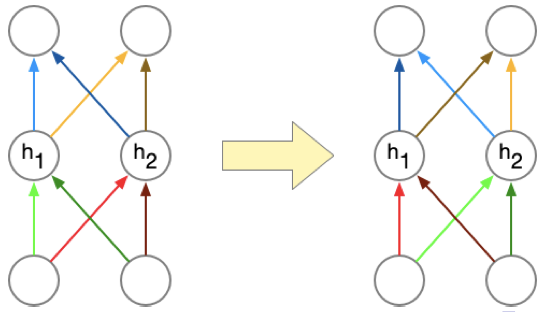
\includegraphics[width=0.45\textwidth]{img/net_permutation}
\end{figure}
\paragraph{Multilayer Neural Net Non-Convex Argument}
\begin{itemize}
    \item By definition, if a (cost) function $\mathcal{J}$ is convex, then for any set of points $\boldsymbol{\theta}_{1}, \dots, \boldsymbol{\theta}_{N}$ in its domain, we know
    \begin{equation}
        \mathcal{J}\left(\lambda_{1} \boldsymbol{\theta}_{1}+\cdots+\lambda_{N} \boldsymbol{\theta}_{N}\right) \leq \lambda_{1} \mathcal{J}\left(\boldsymbol{\theta}_{1}\right)+\cdots+\lambda_{N} \mathcal{J}\left(\boldsymbol{\theta}_{N}\right) \quad \text { for } \lambda_{i} \geq 0, \sum_{i} \lambda_{i}=1
    \end{equation}
    \item Due to permutation symmetry, there are $K!$ (where $K$ is the number of hidden units in a given hidden layer) permutations of the hidden units in a given layer which all compute the same function. 
    \item Suppose that we average the parameters for all $K!$ permutations, then we get a degenerate network where all the hidden units are identical (i.e. the network learnt nothing using these identical weights).
    \item Under the assumption that the cost function was convex, this solution would have to be better than the original one (i.e. the one before we average out all the weights in hidden units) and this leads to a contradiction.\footnote{Remark: Generally, it is safe to say that a network that has leant\textit{\textbf{ absolutely nothing }}would have a much higher cost than a network that, at least, converged to a local minimum} \contradiction Thus training a multilayer neural nets is non-convex.\qed
\end{itemize}

\subsection{Nuisance-ness of Cost Surface}
In this sub-section, we will discuss how non-nice 
\subsubsection{Saddle Point}
A saddle point is a point if
\begin{itemize}
    \item $\nabla \mathcal{J}(\boldsymbol{\theta})=\mathbf{0}$, and
    \item $\mathbf{H}(\boldsymbol{\theta} )$ has some positive and some negative eigenvalues, i.e. some directions with positive curvature and some with negative curvature. 
\end{itemize}
This could be troublesome since
\begin{itemize}
    \item If we are exactly on the saddle point, then we are stuck - gradient descent won't get us any further.
    \item In such case, if we inspect the cost, we would judge that the algorithm has converged. However the solution acquired could be far from optimal. 
\end{itemize}
We can tackle this problem by perturbing the current weight solution slightly in the weight space so that the weight could start moving again. It is important that we don't initialize all of the weights to zero, we should break the symmetry by using small random values. 

\subsubsection{Plateaux}
Plateaux happen more than we think they do, here are some examples that very common
\begin{itemize}
    \item 0-1 loss
    \item hard threshold activations
    \item logistic activations and least square
\end{itemize}
\paragraph{Saturated Unit} is when we are in the flat region of the activation function. In the case of logistic non-linearity ($y = 1/(1 + e^{-x})$), when we have very large or very small $x$'s the gradient would be very close to zero and thus the weights update will get stuck (or be extremely slow).   
\paragraph{Dead Unit} describes an even more extreme case where the gradient is exactly zero. For example, the negative half of the ReLU activation. 

\subsubsection{Ill-Conditioned Curvature}\footnote{This is very common in neural net training.}
Below is a typical example\cite{week4} of a Ill-conditioned curvature
\begin{figure}[H]
    \center 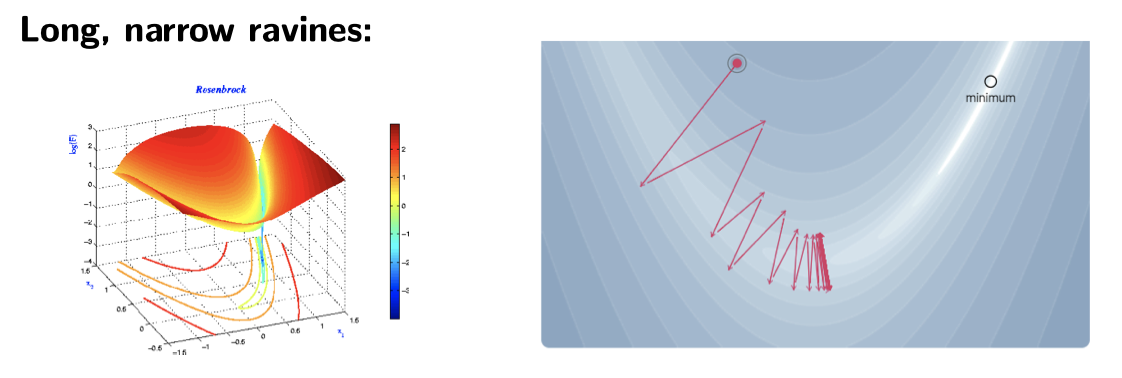
\includegraphics[width=0.75\textwidth]{img/ravine}
    \advance\leftmargini 2em
    \advance\rightmargin 2em
    \begin{quotation}
        As we can see from the gradient updates shown in the level set graph, the solution that we get at each iteration bounces back and forth in the high curvature directions and makes very minimal progress in the low curvature direction. 
    \end{quotation}
\end{figure}
\noindent We can characterize such curvature by noticing that the hessian $\mathbf{H}$ would have some \textit{large} positive eigenvalues and some eigenvalues close to zero, corresponding to high-curvature and low-curvature directions respectively.

\paragraph{Gradient Descent Dynamics}
Consider a quadratic objective (which is convex)
\begin{equation}
    \mathcal{J}(\boldsymbol{\theta})=\frac{1}{2} \boldsymbol{\theta}^{\top} \boldsymbol{A} \boldsymbol{\theta} \quad\quad \text{where $\mathbf{A}$ is $+$-ive semi definite}
\end{equation}
then the gradient descent updates would be 
\begin{align}
    \boldsymbol{\theta}_{k + 1} 
    &\gets \boldsymbol{\theta}_k - \alpha \nabla \mathcal{J} (\boldsymbol{\theta}_k) \\
    &= \boldsymbol{\theta}_k - \alpha \mathbf{A} \boldsymbol{\theta}_k \\
    &= (\mathbf{I} - \alpha \mathbf{A})\boldsymbol{\theta}_k \\
    \implies \boldsymbol{\theta}_k &= (\mathbf{I} - \alpha \mathbf{A})^k \boldsymbol{\theta}_0
\end{align}
Let $\mathbf{A} = \mathbf{Q} \wedge \mathbf{Q}^{\top}$ be the spectral decomposition of $\mathbf{A}$, then
\begin{align}
    (\mathbf{I}-\alpha \mathbf{A})^{k} \boldsymbol{\theta}_{0}
    &=\left(\mathbf{I}-\alpha \mathbf{Q} \mathbf{\Lambda} \mathbf{Q}^{\top}\right)^{k} \boldsymbol{\theta}_{0} \\
    &=\left[\mathbf{Q}(\mathbf{I}-\alpha \boldsymbol{\Lambda}) \mathbf{Q}^{\top}\right]^{k} \boldsymbol{\theta}_{0} \\
    &= \mathbf{Q}(\mathbf{I}-\alpha \boldsymbol{\Lambda})^{k} \mathbf{Q}^{\top} \boldsymbol{\theta}_{0} && \text{$\mathbf{Q}$ is orthonormal, thus $\mathbf{Q}^\top\mathbf{Q} = \mathbf{I}$} \\
    &= \mathbf{Q}(\mathbf{I}-\alpha \boldsymbol{\Lambda})^{k} \mathbf{Q}^{-1} \boldsymbol{\theta}_{0}
\end{align}
In $\mathbf{Q}$ basis, each coordinate gets multiplied by $\left(1-\alpha \lambda_{i}\right)^{k}$ where $\lambda_i$'s denote eigenvalues of $\mathbf{A}$. Hence, 
\begin{itemize}
    \item If $0 < \alpha \lambda_i \leq 1$: decays to zero at a rate that depends on $\alpha \lambda_i$
    \item If $1 < \alpha \lambda_i \leq 2$: oscillations will happen
    \item If $\alpha \lambda_i > 2$: then the gradient updates diverges. (unstable)
\end{itemize}
The result is that we will need to set our learning rate such that
\begin{equation}
    \alpha < \frac{2}{\lambda_{\max}} \quad\quad\quad \text{where}\, \lambda_{\max} \triangleq \max_i \lambda_i
\end{equation}
to prevent instability (divergence). Notice that the goal here is to prevent divergence rather than preventing oscillations, this is why we have the 2 on the numerator. We can bound the rate of convergence in another direction, 
\begin{equation}
    \alpha \lambda_{i}<\frac{2 \lambda_{i}}{\lambda_{\max }}
\end{equation}
We call $\lambda_{\max} / \lambda_{\min}$ as \textit{\textbf{condition number}} of $\mathbf{A}$. The larger the condition number, the slower the convergence of gradient, vice versa. Notice that $\lambda_{\max} / \lambda_{\min}$ is large when the difference between the largest smallest eigenvalue is large, i.e. the curvatures have a large difference and this is trouble-some for gradient decent updates. 

\paragraph{Normalization} In the case that we have ravine-like cost surfaces, gradient updates could have a lot of bouncing around. Even more annoyingly, gradient descent updates will calculate a larger update along the direction with steeper gradient, which in the case of ravine will almost certainly cause the gradient updates to overshoot. To overcome this, we introduce normalization, i.e. centring inputs to zero mean and unit variance. This is especially necessary when we have mixed units in inputs. The normalization we apply is
\begin{equation}
    \tilde{x}_{j}=\frac{x_{j}-\mu_{j}}{\sigma_{j}}
\end{equation}
Notice that if we want to normalize all the outputs of all the layers (including hidden layers) then we can't just normalize the output to have a mean of zero. This is due to the fact that our activations are (usually) non-zero centred, for example logistic non-linearity.
\begin{itemize}
    \item The first trick that we can use is to replace logistic non-linearity with $\tanh$ which is also a sigmoid function, but ranges from $-1 to 1$ and thus have a zero centre. 
    \item A recent method called \textit{\textbf{batch normalization}} explicitly centres each hidden activation. In practice, it often speeds up training by 1.5 to 2 times!
\end{itemize}

\subsection{Alternative Gradient Descent}
\subsubsection{Momentum Gradient Descent}
To deal with ill-conditioned curvatures, we want to introduce a notion of ``history'' through ``acceleration accumulated along the way'' in our gradient descent updates. The updates are
\begin{align}
    \mathbf{p} &\gets \mu\mathbf{p} - \alpha \partial_{\boldsymbol{\theta}} \mathcal{J} \\
    \boldsymbol{\theta} &\gets \boldsymbol{\theta} + \bp
\end{align}
where $\alpha$ is the usually learning rate, and $\mu$ is called a damping parameter and should be some value less than 1 (typically 0.99 or 0.9). Intuitively, this is the ``history decay rate'' and if we have $\mu = 1$ then since we have no decay of energy through time, by conservation of energy the updates will never settle down. (which is bad, we don't want this)
\begin{itemize}
    \item In the high curvature directions, the gradients cancel each other out, so momentum dampens the oscillations, 
    \item In the low curvature directions, the gradient point in the same direction, allowing the parameters to ``pick up speed''.
    \item \textit{\textbf{\#! Important:}} If you increase $\mu$, you should lower $\alpha$ to compensate. Here is a demonstration for the case where gradient is constant. In such case, 
        \begin{align}
            \bp &= -\alpha \partial_{\boldsymbol{\theta}}\mathcal{J} \\
            \implies \bp_1 &= \mu \bp_0 - \alpha \partial_{\boldsymbol{\theta}} \mathcal{J} = - \alpha \mu \partial_{\boldsymbol{\theta}} \mathcal{J} - \alpha \partial_{\boldsymbol{\theta}} \mathcal{J} \\
            \implies \bp_2 &= - \alpha\mu^2 \partial_{\boldsymbol{\theta}} \mathcal{J} - \alpha\mu \partial_{\boldsymbol{\theta}} \mathcal{J} - \alpha \partial_{\boldsymbol{\theta}} \mathcal{J} \\
            \implies \bp_k &= -\alpha \left(\sum_{i = 1}^k \mu^i\right) \partial_{\boldsymbol{\theta}} \mathcal{J} \overset{k\rightarrow\infty}{\rightsquigarrow} \frac{-\alpha}{1 - \mu} \partial_{\boldsymbol{\theta}} \mathcal{J}
        \end{align}
    Thus, if we want to ``keep'' the optimal velocity of approaching optimal spot, we will need to keep a balance between $\mu$ and $\alpha$. \qed
\end{itemize}



\subsubsection{Stochastic Gradient Descent}
The sort of gradient descent that updates each step using the entire training dataset is called \textit{\textbf{batch training}}. Alternative to that we can use SGD which updates the parameters based on the gradient for one single training example, i.e.
\begin{equation}
    \boldsymbol{\theta} \leftarrow \boldsymbol{\theta}-\alpha \nabla \mathcal{J}^{(i)}(\boldsymbol{\theta})
\end{equation}
this allows the training to make a lot of progress before seeing all the training data. As the name suggest, this of course will introduce noise, we can show that SGD gives unbiased estimate of the batch gradient, 
\begin{equation}
    \mathbb{E}_{i}\left[\nabla \mathcal{J}^{(i)}(\boldsymbol{\theta})\right]=\frac{1}{N} \sum_{i=1}^{N} \nabla \mathcal{J}^{(i)}(\boldsymbol{\theta})=\nabla \mathcal{J}(\boldsymbol{\theta})
\end{equation}

\subsubsection{Minibatch SGD}
The problem with SGD with one single training example at a time is that we can't vectorize operations and thus we can't exploit efficient vectorized operations. As a compromise, we can use mini-batch at each update, typically of size $|\mathcal{M}| = S = 100$. 
\begin{itemize}
    \item We call one pass through the \textit{entire dataset} as a \textbf{\textit{epoch}}. 
    \item Larger mini-batches will have smaller variance, 
        \begin{equation}
            \operatorname{VAR}\left[\frac{1}{S} \sum_{i=1}^{S} \frac{\partial \mathcal{L}^{(i)}}{\partial \theta_{j}}\right]=\frac{1}{S^{2}} \operatorname{VAR}\left[\sum_{i=1}^{S} \frac{\partial \mathcal{L}^{(i)}}{\partial \theta_{j}}\right]=\frac{1}{S} \operatorname{VAR}\left[\frac{\partial \mathcal{L}^{(i)}}{\partial \theta_{j}}\right]
        \end{equation}
    \item If we choose to have larger batches,  then the algorithm will converge using fewer weight updates since increasing batch size decreases the stochasticity. Otherwise, if we choose to have small batches, we will be able to perform more weight updates per second because update operations are now cheaper. 
    \item \textit{\textbf{\#! Important:}} If actual time is proportional to FLOPs\footnote{Floating Point Operations per second} that a processor can handle, then $S =1$ is optimal.
    \begin{itemize}
        \item Under this assumption, 100 updates with $S = 1$ and 1 update with $S = 100$ will require the same amount of operations and thus will require a same amount of time. 
        \item Clearly, holding everything else equal, we would prefer to have gradients for fresh values of parameter by using 100 updates rather than 1 update. \note{Of course, the $S = 100$ update would be less noisy, but $100$ steps, albeit stochasticity, would almost certainly go further than one step. }
    \end{itemize}
    \item The batch size of choice strong depends on the hardware that the algorithm was running on\cite{week4}
    \begin{figure}[H]
        \center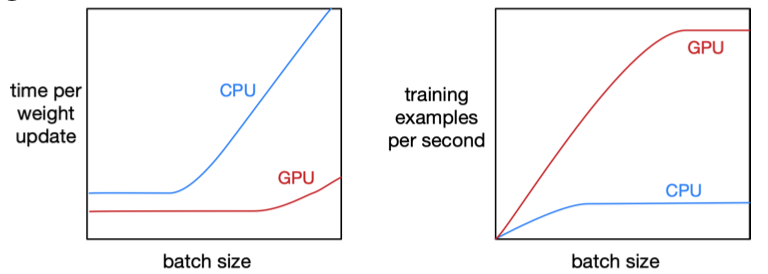
\includegraphics[width=0.6\textwidth]{img/parallel_flops}
    \end{figure}
\end{itemize}

\subsubsection{SGD Learning Rate}
\begin{itemize}
    \item In stochastic training, the learning rate also influences the fluctuations due to the stochasticity of the gradients. 
    \item In practice, we use a large learning rate early in training to that we can converge faster and then gradually decay the learning rate to reduce the fluctuations at the end of training. 
    \item Notice that by reducing learning rate, we will reduce fluctuations, which can appear to make the loss drop suddenly. However, this can come at the expense of long run performance. \cite{week4}
        \begin{figure}[H]
            \center 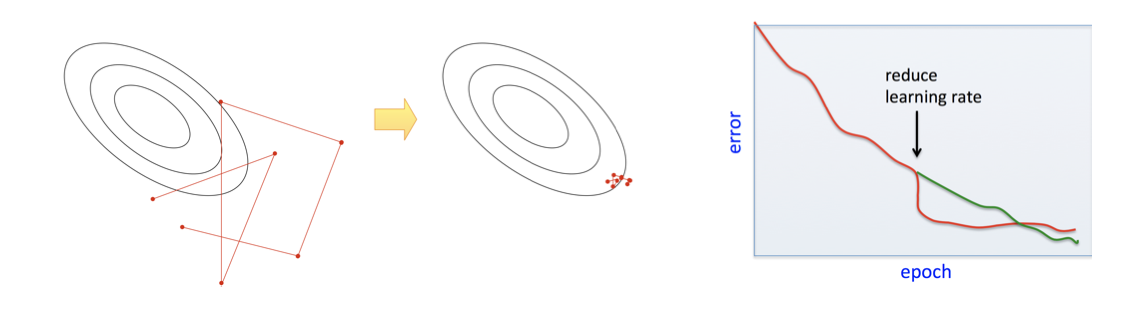
\includegraphics[width=0.75\textwidth]{img/sgd_lr}
        \end{figure}
\end{itemize}

% Focusing on how to tune training hyper-parameters
\subsection{Debugging Optimization}
Here is a table that summarizes different problems that we might encounter during training time, and how to can tackle them \cite{week4}
\begin{figure}[H]
    \center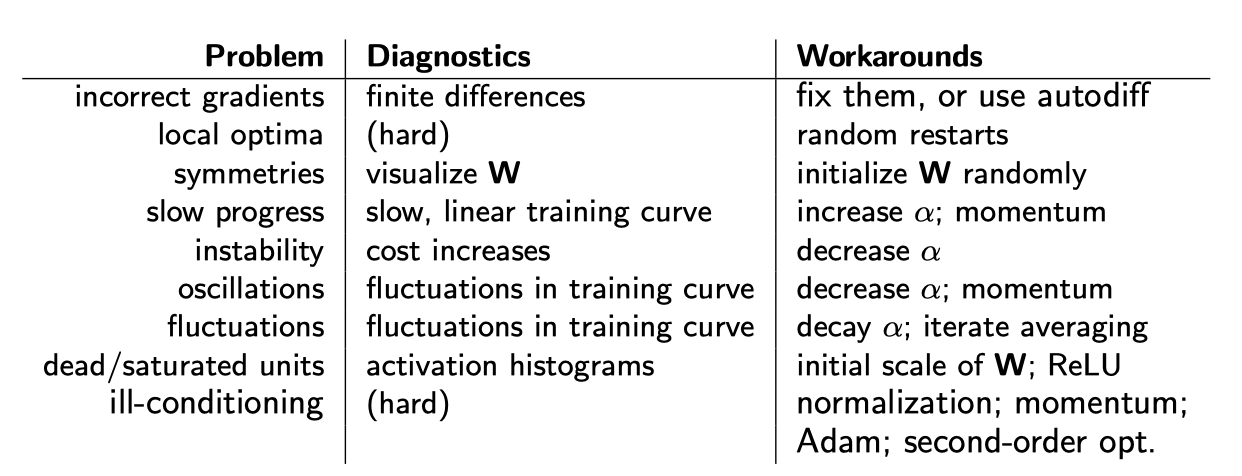
\includegraphics[width=0.7\textwidth]{img/training_problems}
\end{figure}












\section{Convolutional Neural Net and Image Classification}
\subsection{Motivations for Convolution Layer}
\begin{itemize}
    \item Images are, usually, large and hence using a lot of fully connected layers would result in an insane amount of parameter to learn and makes calculation intractable.
    \item In images, there are usually \textit{local} patterns or relationships. For example in the task of semantic segmentation, usually the pixel at bottom left has very little to do with the pixel at top right and using a fully connected layer where every pixel contributes to every output would be wasteful. Thus, we want to have an operation that focus on \textit{\textbf{local}} patterns of the input image.
    \item Also, the same sorts of features that are useful in analyzing one part of the image will probably be useful for analyzing other parts of the image as well which motivates us in using a ``filter'' to ``slide'' across the input. 
\end{itemize}

\subsection{The Convolution Operator}
\subsubsection{1-D Signal Processing} Consider two arrays, $a$ and $b$. The result of the convolution will be a new array, where\note{In order to make this indexing notation to work, we have to have the indices start at zero rather at one. }
\begin{equation}
    (a * b)_{t}=\sum_{\tau} a_{\tau} b_{t-\tau}
\end{equation}
Here the summation over $\tau$ is a lazy notation for saying summing over all combinations that makes sense. \footnote{We assume infinite zero padding here, more on this later.}

\subsubsection{2-D Convolution}
Consider two two dimensional arrays, $A$ and $B$. The result of the convolution will be such that the slot at $(A\ast B)_{ij}$ is calculated as
\begin{equation}
    (A * B)_{i j}=\sum_{s} \sum_{t} A_{s t} B_{i-s, j-t}
\end{equation}
Usually, we call the matrix/tensor that we convolve the original input with a ``kernel'' or ``filter''. 

\subsubsection{Properties of Convolution}
\begin{itemize}
    \item Convolution is \textit{\textbf{Commutative}}, i.e.,
        \begin{equation}
            a * b=b * a
        \end{equation} 
    \item Convolution is \textit{\textbf{Linear}}, i.e., 
        \begin{equation}
            a *\left(\lambda_{1} b+\lambda_{2} c\right)=\lambda_{1} a * b+\lambda_{2} a * c
        \end{equation}
\end{itemize}

\subsection{Canonical Kernels}\change{Some of these canonical kernels are not working as expected...}
\subsubsection{Blurring Kernel}
\begin{equation}
    \begin{array}{|c|c|c|}
        \hline 0 & {1} & {0} \\
        \hline 1 & {4} & {1} \\
        \hline 0 & {1} & {0} \\
        \hline
    \end{array}
\end{equation}

\subsubsection{Sharpening Kernel}
\begin{equation}
    \begin{array}{|c|c|c|}
        \hline 0 & {-1} & {0} \\
        \hline -1 & {5} & {-1} \\
        \hline 0 & {-1} & {0} \\
        \hline
    \end{array}
\end{equation}

\subsubsection{Edge Detector Kernel}
\begin{equation}
    \begin{array}{|c|c|c|}
        \hline 0 & {-1} & {0} \\
        \hline-1 & {4} & {-1} \\
        \hline 0 & {-1} & {0} \\
        \hline
    \end{array}
\end{equation}

\subsubsection{Vertical Edge Detector Kernel}
    \begin{equation}
        \begin{array}{|c|c|c|}
        \hline 1 & {0} & {-1} \\
        \hline 2 & {0} & {-2} \\
        \hline 1 & {0} & {-1} \\
        \hline
    \end{array}
\end{equation}

\subsection{Convolutional Networks}
In a Convolutional Neural Net, of course there will be convolution layers, however there is another sort of layers that are common, called the pooling layer. Intuitively, pooling layers shrink the dimensions by taking a ``local pool''.
\subsubsection{Pooling Layer}
Most commonly, we use the max-pooling operation in the pooling layer, which computes the maximum of the units in a pooling group
\begin{equation}
    y_i = \overset{\max}{j \text{in local pooling group}}z_j
\end{equation}
where $z$ represents the input and $y$ is the output. Typically, we use a $2\times 2$ max pooling unit, which outputs
\begin{equation}
    \begin{array}{|c|c|}
        \hline
        \alpha & \beta \\
        \hline
        \gamma & \theta \\
        \hline
    \end{array} 
    \quad \longrightarrow
    \quad
    \begin{array}{|c|}
        \hline
            \max\{\alpha, \beta, \gamma, \theta\} \\
        \hline
    \end{array}
\end{equation}
Thanks to pooling layers, deeper layers' filters will cover a larger region of the input than equal-sized filters in the lower layers. We say that deeper pooling layers have larger receptive fields in terms of the original image. 

\subsubsection{Non-linearity in Convolutional Layers}
After convolution operation, it is common to add a non-linear activation function to introduce non-linearity. We are doing this because convolution is a linear operation and stacking convolution layers together without non-linearity is no more powerful than a single linear layer (possibly a fully connected layer). For example, the order of the layers could be
\begin{equation}
    \text{Image} \rightarrow \underbrace{\text{Convolution} \rightarrow \text{ReLU activation}}_{\text{Convolution Layer}} \rightarrow \text{Max Pooling} \rightarrow \text{Convolution} \rightarrow \cdots
\end{equation}

\subsubsection{Equivariance and Invariance}
\todo[inline]{TODO: I have no idea...}
We want our network's responses to be robust to translations of the input, which could mean the following two things
\begin{itemize}
    \item Convolution layers are equivariant\footnote{Equivariant means roughly``unchanged in terms of distortion''}: if you translate the inputs, the outputs are translate by the same amount. 
    \item Network's predictions are invariant: if you translate the inputs, the prediction should not change. Pooling layers provide invariance to small translations. 
\end{itemize}

\subsubsection{Channels in Convolution Layers}
Each layer is consist of several feature maps, or \textit{\textbf{channels}}, each of which is an array (and of the same size). In the case where input is an image, then usually we would have 3 channels for coloured input (RGB channels) and 1 channel if it is in greyscale. Each unit is connected to each unit within its receptive field in the previous layer. This includes \textit{all} of the previous layer's feature maps. 

\subsection{Size of Convolutional Neural Nets}
There are several ``measures of sizes'' that are interested in, namely
\begin{itemize}
    \item \textit{\textbf{Number of units:}} measures the activations needed to be stored in memory during training for back propagation.
    \item \textit{\textbf{Number of weights:}} since weights need to be stored (and updated at each iteration) in memory. 
    \item \textit{\textbf{Number of connections:}} measures the computation costs; approximately 3 add-multiply operations per connection. (1 for the forward pass, and 2 for backward pass.)
\end{itemize}
Below is the number of parameters in a fully connected multilayer perceptron layer along side with those in a convolutional layer. \cite{convNetSize}
\begin{figure}[H]
    \center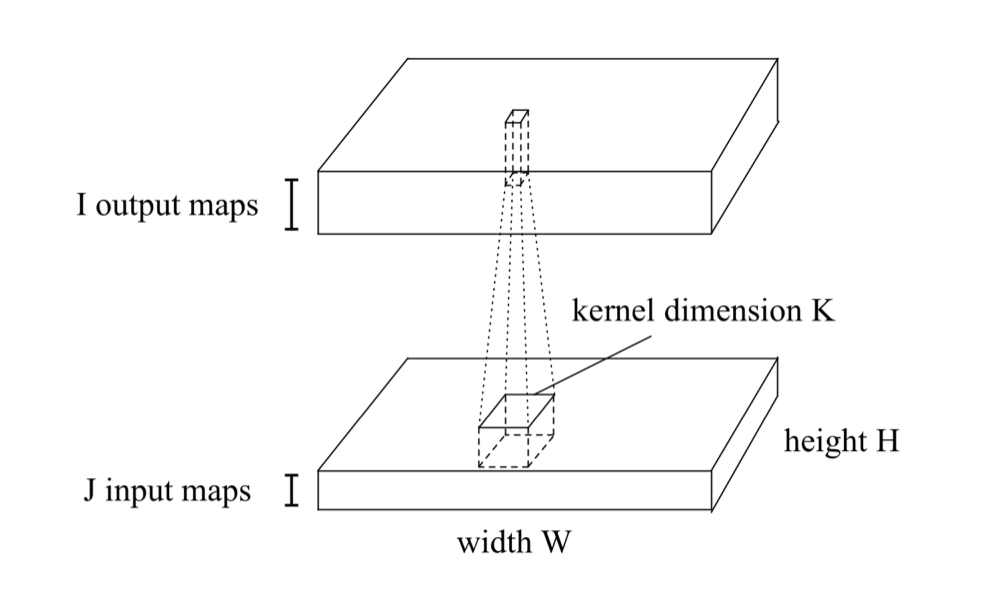
\includegraphics[width=0.75\textwidth]{img/size_conv_net}
\end{figure}
\begin{center}
    \begin{tabular}{c||c|c|}
        & fully connected layer & convolution layer \\
        \hline \hline
        \# output units & $WHI$ & $WHI$ \\
        \hline 
        \# weights & $W^2H^2IJ$ & $K^2IJ$ \\
        \hline
        \# connections & $W^2H^2IJ$ & $WHK^2IJ$ \\
        \hline
    \end{tabular}
\end{center}

\subsubsection{Rule of thumb on size}
\begin{itemize}
    \item Most of the units and connections are in the convolution layers, and
    \item Most of the weights are in the fully connected layers. 
\end{itemize}

\subsection{Supervised Pre-training and Transfer Learning}
\begin{itemize}
    \item In practice, we don't usually train an image classifier from scratch since it is unlikely hat we will have millions of cleanly labeled images for our specific datasets. 
    \item If we want to do a computer vision task, it is common to just ``fine-tune'' a pre-trained convolutional neural net on ImageNet or OpenImage. 
    \item We will fix most of the weights in the pre-trained network. Only the weights in the last layer will be randomly initialized and learnt on the current dataset/task. 
\end{itemize}
\paragraph{Fine-tune, how?}
\begin{itemize}
    \item This depends on how many training examples do we have in the new dataset. For example, if we have fewer ew examples, then we can fix more weights from the pre-trained networks and only train a small subset of all weights. Of course, vice versa. 
    \item This also depends on how similar is the new dataset to the dataset that our pre-trained model was trained on. That is, we need `more' fine-tuning if they have dissimilar datasets.
    \item \textit{\textbf{\#! Important:}} Learning rate for the fine-tuning stage is often much lower than the learning rate used for training from scratch. \unsure{why?}
\end{itemize}


\newpage
\bibliographystyle{unsrt}
\bibliography{ref}
\end{document}
